\documentclass[pdf]{beamer}
\mode<presentation>{} 



\usepackage{hyperref}
\usepackage{pgf}
\usepackage{fancyhdr}
\usepackage{tikz}
\usetikzlibrary{trees}
\usetikzlibrary{arrows,automata}
\usetikzlibrary{automata,positioning}
\usetikzlibrary{shapes}
\usepackage{tikz-qtree,tikz-qtree-compat}
\usepackage{mathtools,enumerate,amssymb}
\usetikzlibrary{patterns}
\usepackage[utf8]{inputenc}
\usepackage[T1]{fontenc}
\usepackage{graphicx}
\usepackage{varwidth}
\usepackage{xcolor}
\usepackage{multicol}
\usepackage{multirow}
\usepackage[export]{adjustbox}
\usepackage{wrapfig}
\usepackage{textcomp}
\usepackage{eso-pic}
\usepackage{pgfornament}
\usepackage[export]{adjustbox}



\newcommand\PlaceText[3]{%
\begin{tikzpicture}[remember picture,overlay]
\node[outer sep=0pt,inner sep=0pt,anchor=south west] 
  at ([xshift=#1,yshift=-#2]current page.north west) {#3};
\end{tikzpicture}%
}



\usetikzlibrary{arrows,positioning} 
\tikzset{
    %Define style for boxes
    punkt/.style={
           rectangle,
           draw=blue, thick,
           minimum height=2em,
           text centered},
    dreptunghi/.style={
           rectangle,
           draw=black,
           minimum height=2em}
}


\newcommand{\textbox}[5]{
\begin{tikzpicture}
\node[punkt,text width=#2] (market) {\textbf{#1}};
\draw[draw=blue] (market.north east)  +(0.2cm,-0.2) -- +(#3,-0.2cm) -- +(#4,#5) ;
\end{tikzpicture}
}



\title{Metaphors and Direct Manipulation}
\subtitle{Human Computer Interaction}
\AtBeginSection[]{}



\setbeamertemplate{sidebar right}{}
\setbeamertemplate{footline}{%
\hfill\usebeamertemplate***{navigation symbols}
\hspace{1cm}\insertframenumber{}/\inserttotalframenumber}



\definecolor{background}{RGB}{255,255,255}
\setbeamercolor{background canvas}{bg=background}
\setbeamercolor{frametitle}{fg=blue}

\graphicspath{{./img/}}



\begin{document}



{\setbeamercolor{background canvas}{bg=background}
\begin{frame}
\vspace{10mm}
\huge{\raggedleft{\color{black}{\textbf{Metaphors and Direct Manipulation}}}}

\large{\raggedleft{\color{black} Human Computer Interaction}}

\begin{flushright}
\end{flushright}

\fontsize{7pt}{1pt}\selectfont{
Based on slide deck 

\textbf{Part 4: Designing and building visual interfaces. Metaphors and Direct Manipulation}

Human Computer Interaction I: Principles and Design

by

\textbf{Saul Greenberg}
\newline
Professor
\newline
\textbf{University of Calgary, Canada}

\textit{The new slides are marked with a *}
}

\fontsize{5pt}{1pt}\selectfont{ \textcolor{lightgray}
{Slide deck by Saul Greenberg. Permission is granted to use this for non-commercial purposes as long as general credit to Saul Greenberg is clearly maintained.
Warning: some material in this deck is used from other sources without permission. Credit to the original source is given if it is known.}}

\end{frame}}



% Inaintea codului fiecarui slide se vor scrie urmatoarele informatii:
% Nume si prenume student
% Numarul slide-ului corespunzator din prezentarea prof. Saul Greenberg
% Numele imaginilor inserate trebuie sa fie numar_slide_nume_imagine.extensie_imagine



%Ciolacu Iulian-Teodor
%Numarul slide-ului: 1
\definecolor{bluetext}{RGB}{0,0,102}
\definecolor{background}{RGB}{255,255,255}
\setbeamercolor{background canvas}{bg=background}
\begin{frame}
	\bigskip
    \textbf{\LARGE Metaphors and \LARGE}
    \newline
    \textbf{\LARGE Direct Manipulation \LARGE}
   	\newline
    \newline
    \newline
    \textbf{Metaphors}
    \newline
    \textbf{Direct manipulation}
    \newline
    \textbf{Dynamic queries}
\end{frame}



%Ciolacu Iulian-Teodor
%Numarul slide-ului: 2
\definecolor{bluetext}{RGB}{0,0,102}
\definecolor{background}{RGB}{255,255,255}
\setbeamercolor{background canvas}{bg=background}
\begin{frame}
{\textbf{Metaphors in interfaces}}{\textcolor{red}{\rule{12cm}{1.2pt}}}

    \vspace{5px}

   \text{   Pervade excellent interfaces}
   \begin{picture}(0,0)
    \put(-126,-197){\hbox{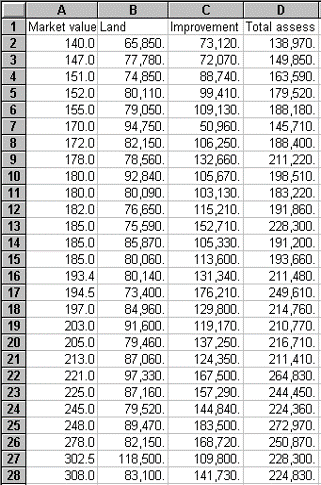
\includegraphics[scale=0.53]{2_Picture1.png}}}
    \end{picture}
     \begin{picture}(0,0)
    \put(16,-101){\hbox{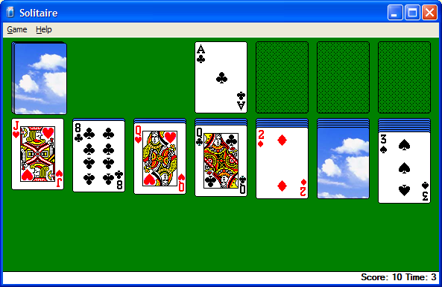
\includegraphics[scale=0.45]{2_Picture2.png}}}
    \put(67,-112){\vspace{100px}\fontsize{8pt}{5pt}\selectfont{\color{black}{games (literal world)}}}
    \end{picture}
    
    \vspace{198px}
    \hspace{25px}\fontsize{8pt}{5pt}\selectfont{\color{black}{spreadsheet (actuary sheet)}} \\
    \AddToShipoutPictureFG*{
    \AtPageLowerLeft{\put(-2,2){\makebox[\paperwidth][r]{\fontsize{4pt}{1pt}\selectfont{\color{gray}{Saul Greenberg}}}}}  
    }
\end{frame}
  
  
  
%Ciolacu Iulian-Teodor
%Numarul slide-ului: 3
\definecolor{bluetext}{RGB}{0,0,102}
\definecolor{background}{RGB}{255,255,255}
\setbeamercolor{background canvas}{bg=background}
\begin{frame}
{\textbf{Metaphors in interfaces}}{\textcolor{red}{\rule{12cm}{1.2pt}}}

\begin{figure}

\includegraphics[scale=0.45]{3_Picture3.png}
\end{figure}

\begin{center}
\textbf{Forms}
\end{center}

\begin{figure}
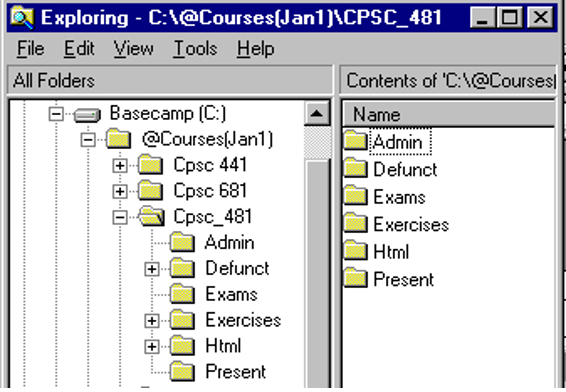
\includegraphics[scale=0.45]{3_Picture1.png}
\end{figure}

\begin{center}
\textbf{Hierarchical folders}
\end{center}
    
\vspace{50px}
\AddToShipoutPictureFG*{
\AtPageLowerLeft{\put(-2,2){\makebox[\paperwidth][r]{\fontsize{4pt}{1pt}\selectfont{\color{gray}{Saul Greenberg}}}}} 
}
\end{frame}



\definecolor{bluetext}{RGB}{0,0,102}
\definecolor{background}{RGB}{255,255,255}
\setbeamercolor{background canvas}{bg=background}
\begin{frame}
{\textbf{Metaphors in interfaces}}{\textcolor{red}{\rule{12cm}{1.2pt}}}

\begin{figure}
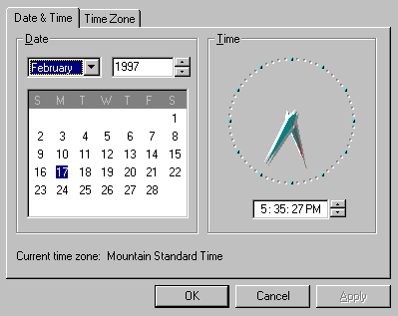
\includegraphics[scale=0.55]{3_Picture2.png}
\end{figure}

\begin{center}
\textbf{Control Panels with familiar control}
\end{center}
    
\vspace{50px}
\AddToShipoutPictureFG*{
\AtPageLowerLeft{\put(-2,2){\makebox[\paperwidth][r]{\fontsize{4pt}{1pt}\selectfont{\color{gray}{Saul Greenberg}}}}} 
}
\end{frame}



%Cioroianu Marius-Rareș
%4
\definecolor{textalbastru}{RGB}{0,0,102}
\definecolor{fundal}{RGB}{255,255,255}
\setbeamercolor{background canvas}{bg=fundal}
\begin{frame}
{\textbf{Metaphors in interfaces}}{\textcolor{red}{\rule{12cm}{1.2pt}}}

  	\text{Definition}
     \begin{itemize}
      \item[--] {represents a system object as if it were another type of object}
      \begin{itemize}
       \item[{$\bullet$}]{ disc / network file structure \textit{represented as} file folders}
      \end{itemize}
    \end{itemize}
    \vspace{10px}
    
    \text{Purpose}
     \begin{itemize}
      \item[--]{ leverages our knowledge of familiar, concrete objects to understand abstract computer and task concepts}
    \end{itemize}
    \vspace{10px}
    
    \text{Problem}
     \begin{itemize}
      \item[--]{metaphor portrays inaccurate/naive conceptual model of the system}
    \end{itemize}
    
    \begin{picture}(0,0)
     \put(50,-30){\hbox{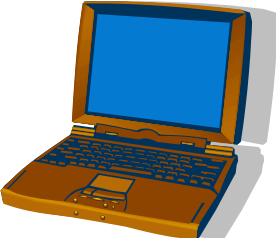
\includegraphics[scale=0.45]{4_Picture1.png}}}
    \end{picture}
    
    \hspace{110px}\fontsize{8pt}{1pt}\selectfont{\color{gray}A presentation tool is a slide projector}
    
    \begin{picture}(0,0)
     \put(250,-10){\hbox{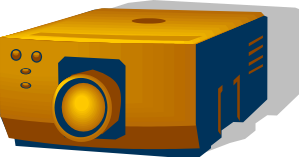
\includegraphics[scale=0.45]{4_Picture2.png}}}
    \end{picture}    
\end{frame}



%Cioroianu Marius-Rareș
%5
\definecolor{textalbastru}{RGB}{0,0,102}
\definecolor{fundal}{RGB}{255,255,255}
\setbeamercolor{background canvas}{bg=fundal}
\begin{frame}
{\textbf{Metaphors in interfaces}}{\textcolor{red}{\rule{12cm}{1.2pt}}}

  	\text{Things to watch for}
    \vspace{10px}
     \begin{itemize}
      \item[--] {Use metaphors that matches user's conceptual task}
      \begin{itemize}
      	\item[--] {desktop metaphor for office workers}
        \item[--] {paintbrush metaphor for artists...}
      \end{itemize}
      \vspace{10px}
      \item[--]{Given a choice, choose the metaphor close to the way the system works}
      \vspace{10px}
      \item[--]{Ensure emotional tone is appropiate to users}
      \begin{itemize}
      	\item[{$\bullet$}] {e.g. file deletion metaphors}
        \begin{itemize}
      	 \item[--] {trashcan}
         \item[--] {black hole}
         \item[--] {paper shredder}
         \item[--] {pit bull terrier}
         \item[--] {nuclear disposal unit...}
      \end{itemize}
      \end{itemize}
    \end{itemize}
    
    \hspace{260px}\fontsize{2pt}{1pt}\selectfont{\color{gray}Saul Greenberg}
    
\end{frame}



%Cioroianu Marius-Rareș
%6
\definecolor{textalbastru}{RGB}{0,0,102}
\definecolor{fundal}{RGB}{255,255,255}
\setbeamercolor{background canvas}{bg=fundal}
\begin{frame}
{\textbf{Metaphors in interfaces}}{\textcolor{red}{\rule{12cm}{1.2pt}}}

    \text{Things to watch for}
    \vspace{10px}
     \begin{itemize}
      \item[--] {will it restrict what people could actually do?}
       \begin{itemize}
       	\item[{$\bullet$}] {strict file/folder hierarchy \newline vs \newline system allows links between directories}
       \end{itemize}
       \vspace{10px}
      \item[--] {will it set unrealistic expectations?}
       \begin{itemize}
       	\item[{$\bullet$}] {Chat-bot}
       \end{itemize}
     \end{itemize}
     
     \vspace{60px}
	 \hspace{260px}\fontsize{2pt}{1pt}\selectfont{\color{gray}Saul Greenberg}
    
\end{frame}



%Plesa Mihail
%Numarul slide-ului:37
\begin{frame}
{\textbf{Metaphors in interfaces}}{\textcolor{red}{\rule{12cm}{1.2pt}}}

\large{ Choosing levels of abstraction }

\bigskip
\bigskip
\bigskip
\bigskip

\begin{figure}
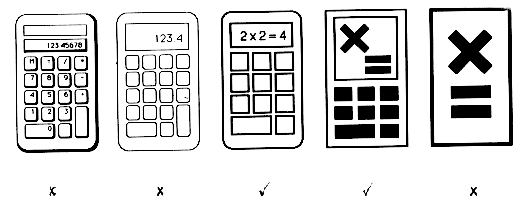
\includegraphics[scale=0.65]{37_picture.png}
\end{figure}
    
    \vspace{145px}
   
    \vspace{35px}
    \AddToShipoutPictureFG*{
    	\AtPageLowerLeft{\put(-2,2){\makebox[\paperwidth][r]{\fontsize{4pt}{1pt}\selectfont{\color{gray}{Saul Greenberg}}}}}
        \AtPageLowerLeft{\put(-310,5){\makebox[\paperwidth][r]{\fontsize{8pt}{1pt}\selectfont{\color{gray}{Mullet \& Sano}}}}}  
    }

\end{frame}



%Cioroianu Marius-Rareș
%7
\definecolor{textalbastru}{RGB}{0,0,102}
\definecolor{fundal}{RGB}{255,255,255}
\setbeamercolor{background canvas}{bg=fundal}
\begin{frame}
{\textbf{Metaphors in interfaces}}{\textcolor{red}{\rule{12cm}{1.2pt}}}

	\text{Common pitfalls}
    \begin{itemize}
      \item[--] {overly literal}
      \begin{itemize}
       	\item[{$\bullet$}] {unnecessary fidelity}
        \item[{$\bullet$}] {excessive interactions}
        \item[{$\bullet$}] {unnecessary restrictions}
       \end{itemize}
       \vspace{10px}
       \item[--] {overly cute}
       \begin{itemize}
       	\item[{$\bullet$}] {novelty quickly wears off}
       \end{itemize}
       \vspace{10px}
       \item[--] {mismatched}
       \begin{itemize}
       	\item[{$\bullet$}] {does not match user's \newline task and/or thinking}
       \end{itemize}
    \end{itemize}
    
    \begin{picture}(0,0)
     \put(155,55){\hbox{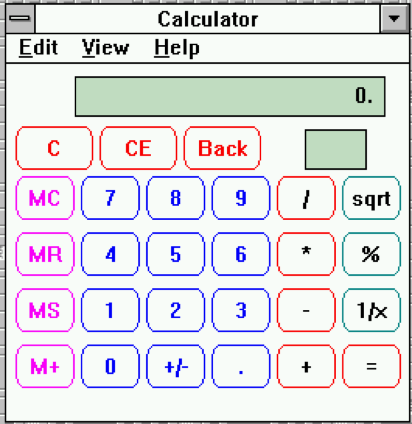
\includegraphics[scale=0.45]{7_Picture1.png}}}
     \put(260,75){\hbox{
\includegraphics[scale=0.45]{6_Picture1.png}}}
     \put(135,-45){\hbox{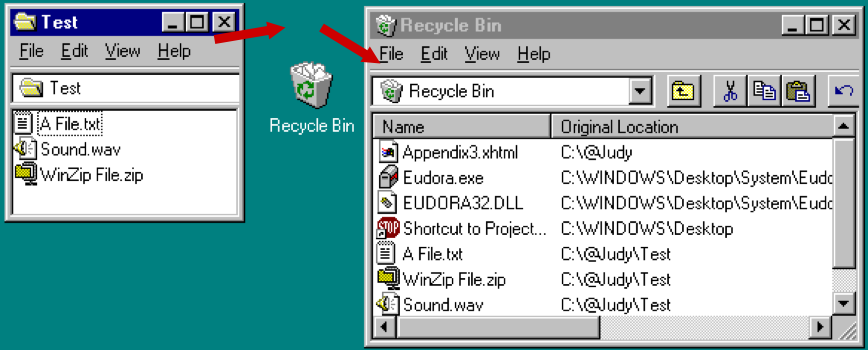
\includegraphics[scale=0.45]{7_Picture2.png}}}
    \end{picture}
    
    \vspace{100px}
    
\end{frame}



%Cioroianu Marius-Rareș
%11
\definecolor{textalbastru}{RGB}{0,0,102}
\definecolor{fundal}{RGB}{255,255,255}
\setbeamercolor{background canvas}{bg=fundal}
\begin{frame}
{\textbf{Metaphor misuses}}{\textcolor{red}{\rule{12cm}{1.2pt}}}

Milltronics' Dolphin Plus - a configuration package for industrial level and flow sensors
    \newline
    
\begin{figure}

\includegraphics[scale=0.45]{11_Picture1.png}
\end{figure}

\end{frame}



\definecolor{bluetext}{RGB}{0,0,102}
\definecolor{background}{RGB}{255,255,255}
\setbeamercolor{background canvas}{bg=background}
\begin{frame}
{\textbf{Direct manipulation}}{\textcolor{red}{\rule{12cm}{1.2pt}}}

Microsoft Solitaire

\begin{figure}
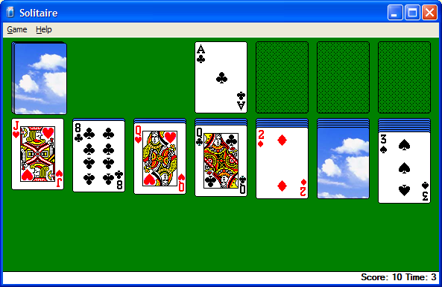
\includegraphics[scale=0.55]{2_Picture2.png}
\end{figure}
    
\text{ \fontsize{14}{10}\selectfont{"A subtle thing happens when everything is visible:} }\\ 	  
\text{ \fontsize{14}{10}\selectfont{the display becomes reality."}} \\
\hspace{180px}
\textit{ \fontsize{14}{10}\selectfont{Xerox Star inventors}} \\
    
\end{frame}



\definecolor{bluetext}{RGB}{0,0,102}
\definecolor{background}{RGB}{255,255,255}
\setbeamercolor{background canvas}{bg=background}
\begin{frame}
{\textbf{Direct manipulation}}{\textcolor{red}{\rule{12cm}{1.2pt}}}

Cropping by drag and drop

\begin{figure}
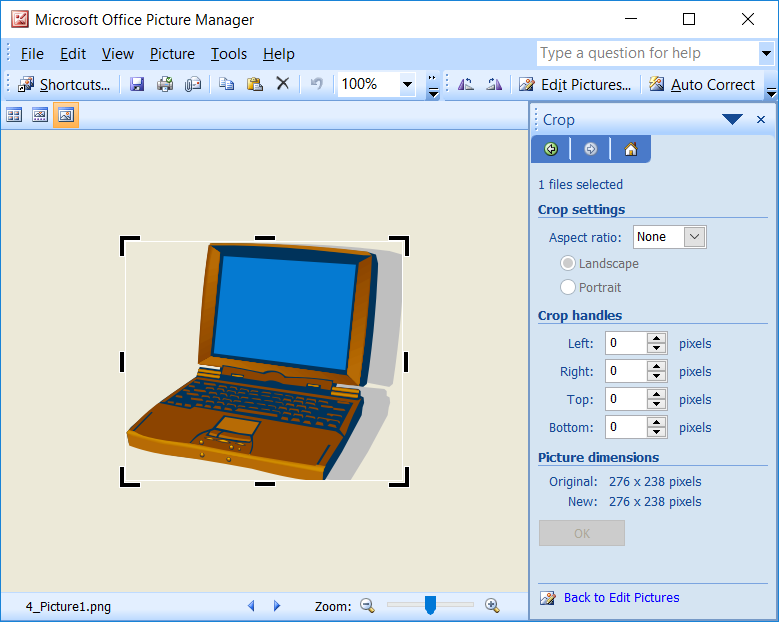
\includegraphics[scale=0.5]{Direct_manipulation_Cropping.png}
\end{figure}
        
\end{frame}



\definecolor{bluetext}{RGB}{0,0,102}
\definecolor{background}{RGB}{255,255,255}
\setbeamercolor{background canvas}{bg=background}
\begin{frame}
{\textbf{Direct manipulation}}{\textcolor{red}{\rule{12cm}{1.2pt}}}

Black Panther film

\vspace{-0.5cm}

\begin{figure}
\centering
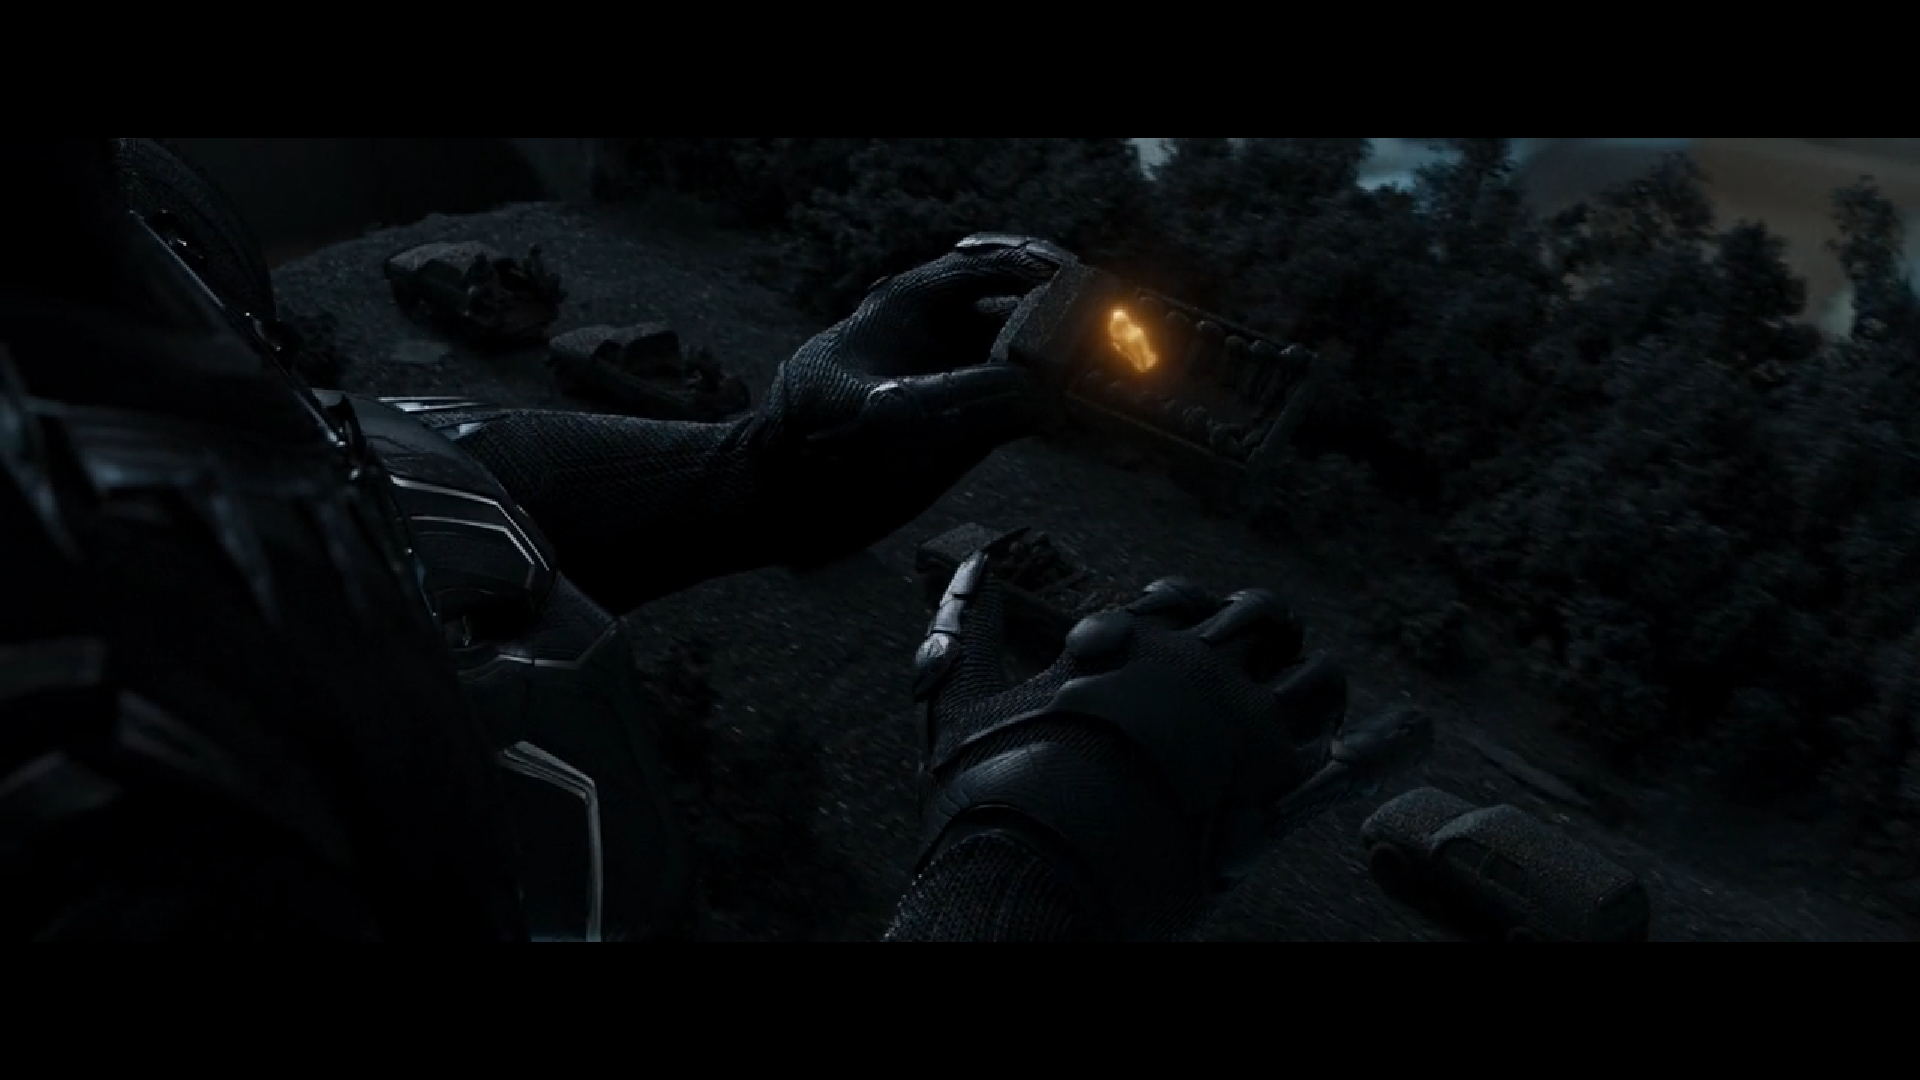
\includegraphics[scale=0.27]{Black_Panther_DM_1.png}
\end{figure}
        
\end{frame}



\definecolor{bluetext}{RGB}{0,0,102}
\definecolor{background}{RGB}{255,255,255}
\setbeamercolor{background canvas}{bg=background}
\begin{frame}
{\textbf{Direct manipulation}}{\textcolor{red}{\rule{12cm}{1.2pt}}}

Black Panther film

\vspace{-0.5cm}

\begin{figure}
\centering
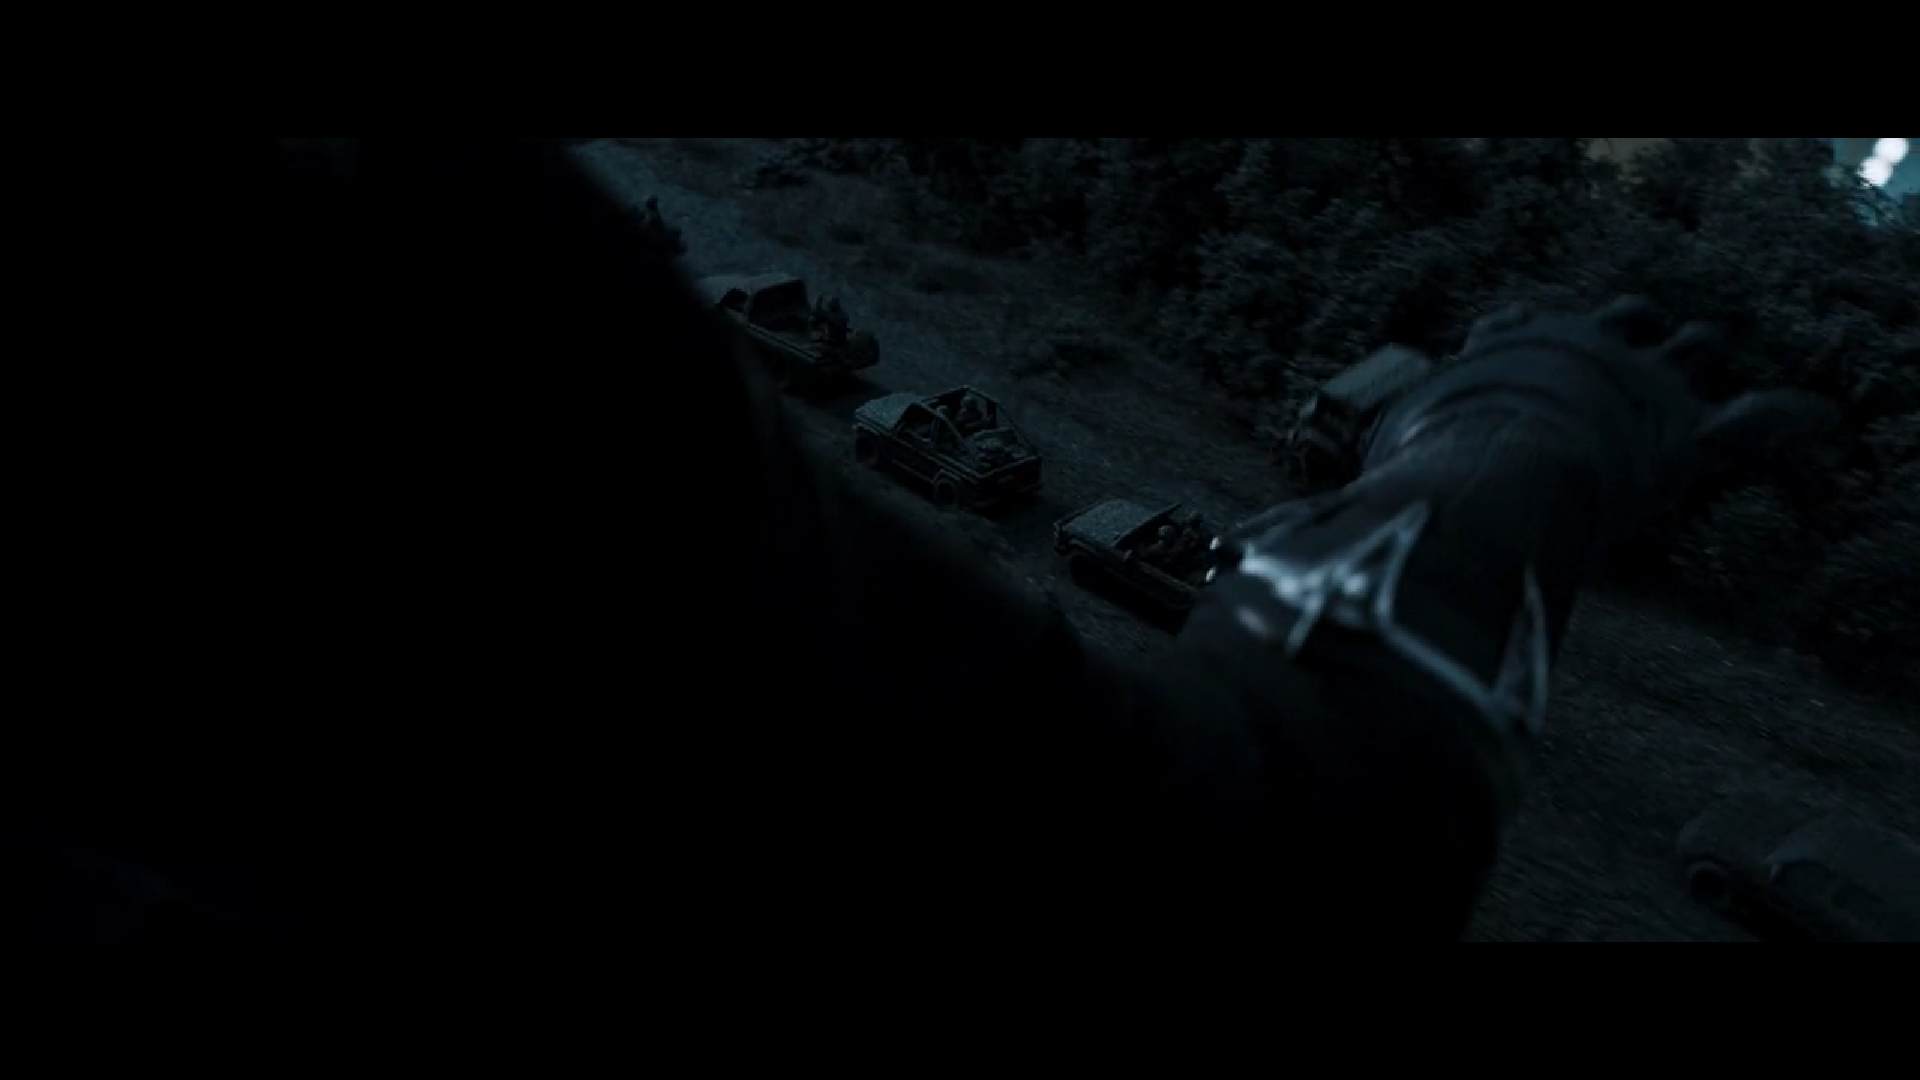
\includegraphics[scale=0.27]{Black_Panther_DM_2.png}
\end{figure}
        
\end{frame}



\definecolor{bluetext}{RGB}{0,0,102}
\definecolor{background}{RGB}{255,255,255}
\setbeamercolor{background canvas}{bg=background}
\begin{frame}
{\textbf{Direct manipulation}}{\textcolor{red}{\rule{12cm}{1.2pt}}}

Black Panther film

\vspace{-0.5cm}

\begin{figure}
\centering
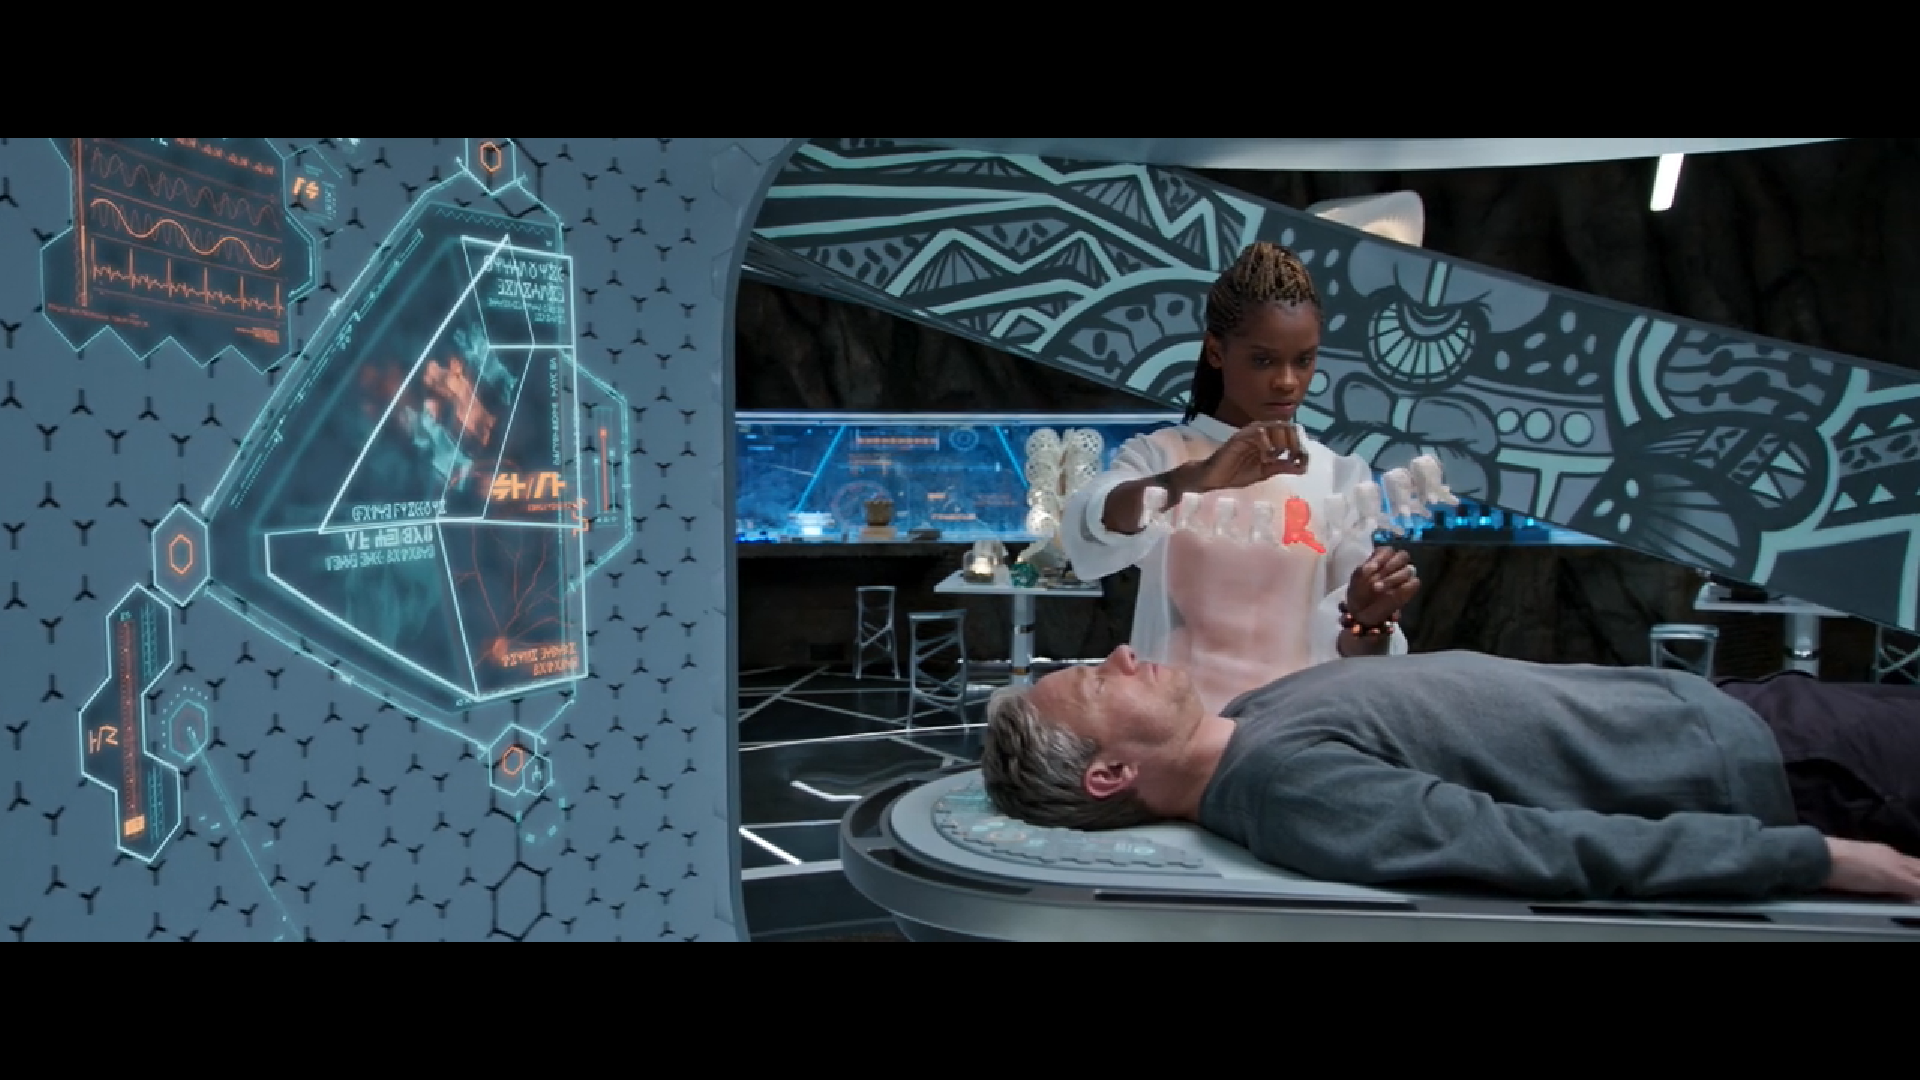
\includegraphics[scale=0.27]{Black_Panther_DM_3.png}
\end{figure}
        
\end{frame}



% Constantinescu Catalin-Stefan
% 12
\definecolor{textalbastru}{RGB}{0,0,102}
\definecolor{fundal}{RGB}{255,255,255}
\setbeamercolor{background canvas}{bg=fundal}
\begin{frame}
{\textbf{Direct manipulation}}{\textcolor{red}{\rule{12cm}{1.2pt}}}

  	\text{Direct Manipulation}
     \begin{itemize}
      \item[--] {interface behaves as though the interaction was with a real-world object rather than with an abstract system}
      \item[--]{ the feeling of working \textit{directly} on the task}
    \end{itemize}
    \vspace{10px}
    
  	\text{Central ideas}
     \begin{itemize}
      \item[--]{ visibility of the objects of interest}
      \item[--]{ rapid, reversible, incremental actions}
      \item[--]{ manipulation by pointing and moving}
      \item[--]{ immediate and continuous display of results (\textit{dynamic queries})}
    \end{itemize}
    \vspace{10px}
    
  	\text{Almost always based on a \textit{metaphor}}
     \begin{itemize}
      \item[--]{ mapped onto some facet of the real world task semantics}
    \end{itemize}
            \AddToShipoutPictureFG*{
    	\AtPageLowerLeft{\put(-2,2){\makebox[\paperwidth][r]{\fontsize{4pt}{1pt}\selectfont{\color{gray}{Saul Greenberg}}}}}  
    }

\end{frame}



% Constantinescu Catalin-Stefan
% 13
\begin{frame}
{\textbf{Direct manipulation}}{\textcolor{red}{\rule{12cm}{1.2pt}}}
    
  	\text{ \fontsize{12}{10}\selectfont{objects understood in terms of their visual characteristics}}
     \begin{itemize}
      	\item[--]{ \fontsize{10}{10}\selectfont{ affordances, constraints}}
      	\newline
     \end{itemize}
    
  	\text{ \fontsize{12}{10}\selectfont{actions understood in terms of their effects on the screen}}
     \begin{itemize}
      	\item[--]{  \fontsize{10}{10}\selectfont{causality}}
      	\newline
     \end{itemize}
    
  	\text{ \fontsize{12}{10}\selectfont{intuitively reasonable actions can be performed at any time}}
     \begin{itemize}
      	\item[--]{  \fontsize{10}{10}\selectfont{conceptual model}}
      	\newline
     \end{itemize}
     
    \vspace{40px}
	    
    \vspace{160px}
    
    \AddToShipoutPictureFG*{
    	\AtPageLowerLeft{\put(-2,2){\makebox[\paperwidth][r]{\fontsize{4pt}{1pt}\selectfont{\color{gray}{Saul Greenberg}}}}}  
    }
\end{frame}



% Constantinescu Catalin-Stefan
% 14
%
\begin{frame}
{\textbf{Object-Action vs Action-Object}}{\textcolor{red}{\rule{12cm}{1.2pt}}}

  	\textbf{\fontsize{12}{10}\selectfont{Select object, \textit{then} do action}}
     \begin{itemize}
     
      	\item[--]{ \fontsize{10}{10}\selectfont{interface emphasizes 'nouns' (visible objects) rather than 'verbs'  (actions)}}
        
     \end{itemize}
     
     
    \begin{picture}(0,0)
    
        \put(220,-40){\hbox{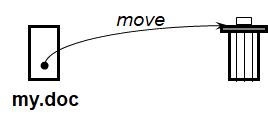
\includegraphics[scale=0.4]{14_Picture.png}}}
        
    \end{picture}
    
  	\textbf{\fontsize{12}{10}\selectfont{Advantages}}
     \begin{itemize}
     
      	\item[--]{ \fontsize{10}{10}\selectfont{closer than real world}}\vspace{-2px}
        
      	\item[--]{ \fontsize{10}{10}\selectfont{modeless interaction}}\vspace{-2px}
        
      	\item[--]{ \fontsize{10}{10}\selectfont{\textit{actions} always within context of object}}\vspace{-2px}
        
        		 \begin{itemize}
                 
                    \item[{•}]{ \fontsize{8}{10}\selectfont{inappropriate ones can be hidden}}\vspace{-2px}
                    
     			\end{itemize}
                
      	\item[--]{ \fontsize{10}{10}\selectfont{\textit{generic commands}}} 
        		 \begin{itemize}
                 
                      \item[{•}]{ \fontsize{8}{10}\selectfont{the same type of action can be performed on the object}} \vspace{-2px}

                      \item[{•}]{ \fontsize{8}{10}\selectfont{eg drag `n drop:}}
                    
                          \begin{itemize}
                          
                                \item[{--}] {\fontsize{8}{10}\selectfont{folders}} \vspace{-2px}

                                \item[{--}] {\fontsize{8}{10}\selectfont{files}} \vspace{-2px}

                                \item[{--}] {\fontsize{8}{10}\selectfont{paragraphs}} \vspace{-2px}

                                \item[{--}] {\fontsize{8}{10}\selectfont{text}} \vspace{-2px}

                                \item[{--}] {\fontsize{8}{10}\selectfont{numbers...}} \vspace{-2px}
                          
     					  \end{itemize}
                          
     			\end{itemize}
                
     \end{itemize}
     
     \vspace{160px}
	 \AddToShipoutPictureFG*{
    	\AtPageLowerLeft{\put(-2,2){\makebox[\paperwidth][r]{\fontsize{4pt}{1pt}\selectfont{\color{gray}{Saul Greenberg}}}}}  
    }
\end{frame}



% Constantinescu Catalin-Stefan
% 16
\begin{frame}
{\textbf{Direct manipulation}}{\textcolor{red}{\rule{12cm}{1.2pt}}}

	Representation affects what can be directly manipulated

	 \begin{picture}(0,0)
        \put(30,-160){\hbox{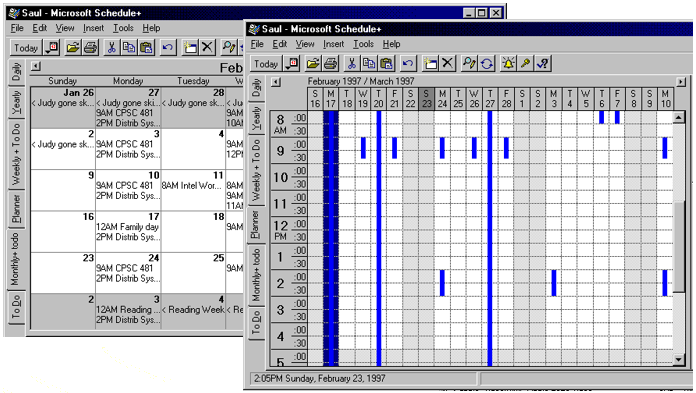
\includegraphics[scale=0.65]{16_picture.png}}}
    \end{picture}

    \vspace{160px}
    \AddToShipoutPictureFG*{
    	\AtPageLowerLeft{\put(-2,2){\makebox[\paperwidth][r]{\fontsize{4pt}{1pt}\selectfont{\color{gray}{Saul Greenberg}}}}}
        \AtPageLowerLeft{\put(-305,5){\makebox[\paperwidth][r]{\fontsize{4pt}{1pt}\selectfont{\color{gray}{Microsoft Schedule+}}}}}  
    }
\end{frame}



%Cornescu Ion Catalin Alexandru
%21
\begin{frame}
{\textbf{Is direct manipulation the way to go?}}{\textcolor{red}{\rule{12cm}{1.2pt}}}
	
{ \fontsize{12}{0}\selectfont{ill-suited for abstract operations}}
 
\vspace{20px}

{ \fontsize{12}{20}\selectfont{tedious}}
  \begin{itemize}
      	\item[--]{ \fontsize{10}{0}\selectfont{manually search large database vs query}}
     \end{itemize}
 
 \vspace{20px}

{ \fontsize{12}{20}\selectfont{solution}}
  \begin{itemize}
      	\item[--]{ \fontsize{10}{0}\selectfont{most systems combine direct manipulation and abstractions}}
        \begin{itemize}
        \item[$\bullet$] { \fontsize{10}{0}\selectfont{word processor:}}
        	\begin{itemize}
        	\item[--] {\fontsize{10}{0}\selectfont{WYSIWYG document (direct manipulation)}}
            \item[--] { \fontsize{10}{0}\selectfont{buttons, menus, dialog boxes (abstractions, but direct manipulation "in the small")}}
        	\end{itemize}
        \end{itemize}
   \end{itemize}
   
\end{frame}



%Cornescu Ion Catalin Alexandru
%22
\begin{frame}
{\textbf{Direct and abstract manipulation}}{\textcolor{red}{\rule{12cm}{1.2pt}}}
    
{\fontsize{12}{0}\selectfont{Most good applications mix the two for power}}

\begin{figure}
        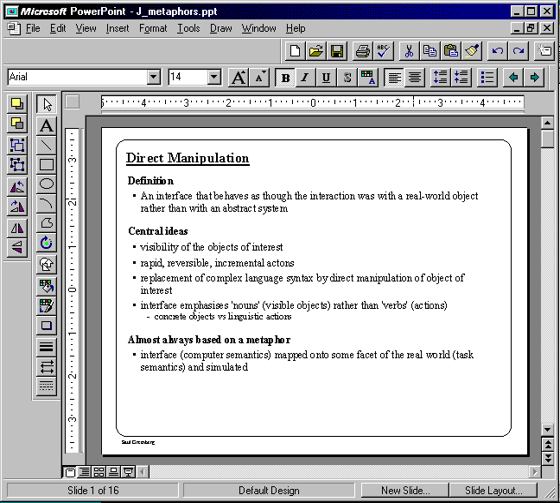
\includegraphics[scale=0.55]{22_Picture1.png}
\end{figure}
   
\end{frame}



%Cornescu Ion Catalin Alexandru
%23
\begin{frame}
{\textbf{Dynamic queries}}{\textcolor{red}{\rule{12cm}{1.2pt}}}

{ \fontsize{12}{20}\selectfont{Searches and queries by}}
  \begin{itemize}
      	\item[--]{ \fontsize{10}{0}\selectfont{adjust sliders, buttons, check boxes, and other control widgets}}
        \item[--]{ \fontsize{10}{0}\selectfont{display immediate updates \textit{as} the control is adjusted
}}
     \end{itemize}
 
 \vspace{20px}

{ \fontsize{12}{20}\selectfont{Why?}}
  \begin{itemize}
      	\item[--]{ \fontsize{10}{0}\selectfont{rapid searching with imprecise queries}}
        \item[--] {\fontsize{10}{0}\selectfont{people explore data interactions and limits}}
        
   \end{itemize}

\end{frame}



%Cornescu Ion Catalin Alexandru
%25
\begin{frame}
{\textbf{HomeBay}}{\textcolor{red}{\rule{12cm}{1.2pt}}}

\vspace{-1cm}    
    
     \begin{picture}(0,0)
        \put(49,-220){\hbox{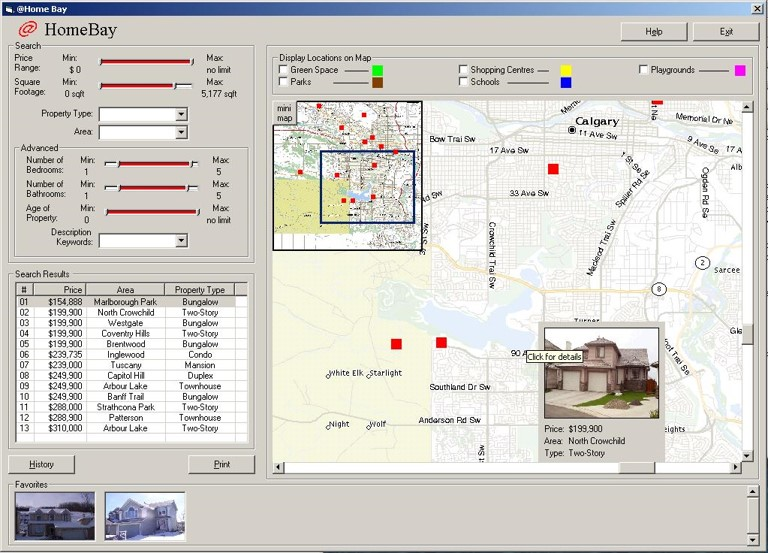
\includegraphics[scale=0.49]{25_Picture1.jpg}}}
    \end{picture}
    
    \vspace{20px}
    {
    \hspace{-32px}{ \vspace{5px} \textbox{Dynamic Queries}{5em}{2}{2.5}{-0.75}}
    
    \hspace{-32px}{\vspace{5px}\textbox{Radar Overview}{5em}{4.6}{5.4}{-0.9}}
    
    \hspace{-32px}{\vspace{5px}\textbox{Progressive details on demand}{5em}{4}{7.65}{-1.4}}}
    
  	\vspace{170px}
   
   \AddToShipoutPictureFG*{
    \AtPageLowerLeft{\put(-110,13){\makebox[\paperwidth][r]{\fontsize{6pt}{1pt}\selectfont{\color{gray}{481 Student Project (April, 2000) Rob Pearson, Kashama Willms and James Chisan}}}}}  
    }
   
\end{frame}



%Cornescu Ion Catalin Alexandru
%27
\begin{frame}
{\textbf{What you now know}}{\textcolor{red}{\rule{12cm}{1.2pt}}}

{ \fontsize{12}{20}\selectfont{Metaphors}}
  \begin{itemize}
      	\item[--]{ \fontsize{10}{0}\selectfont{leverages our knowledge of the familiar and concrete}}
     \end{itemize}
 
 \vspace{5px}

{ \fontsize{12}{20}\selectfont{Direct manipulation}}
  \begin{itemize}
      	\item[--]{ \fontsize{10}{0}\selectfont{visibility of the objects of interest}}
        \item[--] {\fontsize{10}{0}\selectfont{rapid, reversible, incremental actions}}
        \item[--]{ \fontsize{10}{0}\selectfont{manipulation by pointing and moving}}
        \item[--] {\fontsize{10}{0}\selectfont{immediate and continuous display of results (dynamic queries)}}
   \end{itemize}

\end{frame}



%%%% Daca luati slide-ul asta, luati si stilurile definite mai sus
%%%% le gasiti desupra slide-ului 20 - altfel va da eroare la noduri
%%%% si bibloteca tikzarrows deasupra

%primul este latimea
%al 2-lea inaltimea
% al 3-lea paddingul
% la 4 - text width
% al 5-lea este grosimea
% la 6 text
% 7  rotire
% 8 denumire mark
\newcommand{\sageatainsus}[7]{

\begin{tikzpicture}
        \node [single arrow,minimum width=#1, minimum height=#2,draw=black, rotate=#7,line width=#5,inner sep=#3] {   };
        \coordinate (P) at (0,0);
        \node[text width=#4] (N) at (P) {#6} ;
		
\end{tikzpicture}

}


%$ lungime text, grosime dreptunghi, text
\newcommand{\dreptunghi}[3]{

\begin{tikzpicture}
\node[dreptunghi,text width=#1,line width=#2] {#3};
\end{tikzpicture}

}
% culoare, grosime, lungime
\newcommand{\linie}[3]{
\begin{tikzpicture}
\draw[draw=#1,line width=#2] (0,0) -- (0,-#3) ;
\end{tikzpicture}
}


%redefinesc spatiul intre linii
\renewcommand{\baselinestretch}{0.5} 

\begin{frame}
{\textbf{Interface Design and Usability Engineering}}{\textcolor{red}{\rule{12cm}{1.2pt}}}

\vspace{-50px}

%%% poza cu sageti
 \begin{picture}(0,0)
        \put(26,-265){\hbox{
\includegraphics[scale=0.53]{28_Picture1.png}}}
 \end{picture}
 
  %%sagetile lipsa
\begin{picture}(0,0)
\put(118,-242){
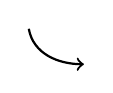
\begin{tikzpicture}
\draw [->,black,line width=0.8] (0,0) to [out=-80,in=180] (0.7,-0.45);
\end{tikzpicture}}
\put(118,-188){
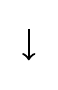
\begin{tikzpicture}
\draw [->,black,line width=0.8] (0,0) to (0,-0.4);
\end{tikzpicture}}

\put(212,-244){
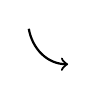
\begin{tikzpicture}
\draw [->,black,line width=0.8] (0,0) to [out=-80,in=180] (0.5,-0.45);
\end{tikzpicture}}
\put(206,-188){
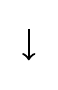
\begin{tikzpicture}
\draw [->,black,line width=0.8] (0,0) to (0,-0.4);
\end{tikzpicture}}
\end{picture}


%%%%% cele 3 lini
% culoare, grosime, plecare (cu minus),lungime

\begin{picture}(0,0)
\put(90,-260){\linie{gray}{3}{8.5}}
\end{picture}


\begin{picture}(0,0)
\put(185,-247){\linie{gray}{3}{8.5}}
\end{picture}

\begin{picture}(0,0)
\put(270,-232){\linie{gray}{3}{8.5}}
\end{picture}

\vspace{-11px}
%%%%%%%%%%%%%%%%%%%partea de sus

\hspace{-29px}\textit{\textbf{\fontsize{9pt}{0pt}\selectfont{\color{black}Goals:
}}}

%primul dreptughi
\begin{picture}(0,0)
\put(20,0)
{\dreptunghi{1.7cm}{0.6}{
\textbf{\fontsize{6pt}{0pt}\selectfont{\color{black}Articulate:\\
\textbullet who users are \\
\textbullet their key tasks
}}}}
\end{picture}


%dreptughiul 2
\begin{picture}(0,0)
\put(122,15)
{\dreptunghi{1.2cm}{0.6}{
\textbf{\fontsize{6pt}{0pt}\selectfont{\color{black}Brainstorm designs
}}}}
\end{picture}

%dreptughiul 3
\begin{picture}(0,0)
\put(212,30)
{\dreptunghi{1.2cm}{0.2}{
\textbf{\fontsize{6pt}{0pt}\selectfont{\color{black}Refined designs
}}}}
\end{picture}

%dreptughiul 4
\begin{picture}(0,0)
\put(285,42)
{\dreptunghi{1.1cm}{0.2}{
\textbf{\fontsize{6pt}{0pt}\selectfont{\color{gray}Completed designs
}}}}
\end{picture}


\vspace{30px}

%%%%%%%%%%%%%%%%%%%partea de mijloc

\hspace{-29px}\textit{\textbf{\fontsize{8.5pt}{0pt}\selectfont{\color{black}Methods:
}}}


%sageata 1
\vspace{20px}
 \begin{picture}(0,0)
 \put(-4,-12){\sageatainsus{5.5em}{7.4em}{4mm}{1.25cm}{0.4}{\fontsize{6pt}{1pt}\selectfont{\color{black}Task centered system \vspace{4px} design 
Participatory  \vspace{4px} design
User-centered design}}{-90}}
 \end{picture}
 
%sageata 2
 \begin{picture}(0,0)
\put(47,7){\sageatainsus{1.8em}{6.8em}{4.5mm}{0.9cm}{0.6}{\fontsize{6pt}{0pt}\selectfont{\color{black} Evaluate tasks}}{90}}
 \end{picture}


%sageata 3
\begin{picture}(0,0)
\put(90,18){\sageatainsus{5em}{7em}{5mm}{1.3cm}{0.4}{
\textbf{\fontsize{6pt}{0pt}\selectfont{\color{black} Psychology of everyday \vspace{4px}  things}}

\fontsize{6pt}{0pt}\selectfont{\color{black} User \vspace{4px} involvement}

\textbf{\fontsize{6pt}{0pt}\selectfont{\color{red} Representation \& metaphors}}
}{-90}}
 \end{picture}
 
 
 %sageata 3 jos
\begin{picture}(0,0)
\put(90,-20){\sageatainsus{5em}{0em}{5mm}{1.2cm}{0.4}{
\textbf{\fontsize{6pt}{0pt}\selectfont{\color{black} low fidelity prototyping methods}}

}{-90}}
 \end{picture}
 
%sageata 4
\begin{picture}(0,0)
\put(137,50){\sageatainsus{4.5em}{7.4em}{5mm}{1.2cm}{0.4}{

\textit{\fontsize{6pt}{0pt}\selectfont{\color{black} Participatory \vspace{8px} interaction}}

\textit{\fontsize{6pt}{0pt}\selectfont{\color{black} Task scenario walk-through
}}

}{90}}
 \end{picture}

%sageata 5
\begin{picture}(0,0)
\put(185,60){\sageatainsus{4em}{7em}{5mm}{1cm}{0.4}{

\fontsize{6pt}{0pt}\selectfont{\color{gray}Graphical screen  \vspace{4px} design}

\fontsize{6pt}{0pt}\selectfont{\color{gray}Interface \vspace{4px} guidelines}

\fontsize{6pt}{0pt}\selectfont{\color{gray}Style  \vspace{4px} guides}

}{-90}}
 \end{picture}
 
 
 %sageata 5 jos
\begin{picture}(0,0)
\put(185,20){\sageatainsus{5em}{4em}{5mm}{1.2cm}{0.4}{
\textbf{\fontsize{6pt}{0pt}\selectfont{\color{black} high fidelity prototyping methods}}

}{-90}}
 \end{picture}

%sageata 6
\begin{picture}(0,0)
\put(228,88){\sageatainsus{4em}{7em}{5mm}{1cm}{0.4}{

\textit{\fontsize{6pt}{0pt}\selectfont{\color{black} Usability
 \vspace{8px} testing}}

\textit{\fontsize{6pt}{0pt}\selectfont{\color{gray} Heuristic evaluation}}
}{90}}
 \end{picture}

%sageata 7
\begin{picture}(0,0)
\put(296,103){\sageatainsus{2.5em}{7em}{3.6mm}{0.7cm}{0.4}{

\textit{\fontsize{6pt}{0pt}\selectfont{\color{gray}Field testing}}
}{90}}
 \end{picture}
 
 
 
 \vspace{-39px}
 %%%%%%%%%%%%%%%%%%%partea de jos

\hspace{-29px}\vspace{25px}\textit{\textbf{\fontsize{9pt}{0pt}\selectfont{\color{black}Products:
}}}

%dreptunghiul 1
\begin{picture}(0,0)
\put(20,27)
{\dreptunghi{1.4cm}{0.2}{
\textbf{\fontsize{6pt}{0pt}\selectfont{\color{black}User and task descriptions
}}}}
\end{picture}

%dreptunghiul 2
\begin{picture}(0,0)
\put(120,40)
{\dreptunghi{1.4cm}{0.2}{
\textbf{\fontsize{6pt}{0pt}\selectfont{\color{black}Throw-away paper prototypes
}}}}
\end{picture}

%dreptunghiul 3
\begin{picture}(0,0)
\put(205,56)
{\dreptunghi{1.2cm}{0.2}{
\textbf{\fontsize{6pt}{0pt}\selectfont{\color{black}Testable prototypes
}}}}
\end{picture}

%dreptunghiul 4
\begin{picture}(0,0)
\put(280,60)
{\dreptunghi{1.4cm}{0.2}{
\textbf{\fontsize{6pt}{0pt}\selectfont{\color{gray}Alpha/beta systems or complete specification
}}}}
\end{picture}
\end{frame}



{\setbeamercolor{background canvas}{bg=background}
\begin{frame}
{\textbf{*Bibliography}}{\textcolor{red}{\rule{12cm}{1.2pt}}}

        \begin{itemize}
        	\item[{$\bullet$}] Saul Greenberg, \textbf{Designing and building visual interfaces. Metaphors and Direct Manipulation}, University of Calgary, Canada

        	\url{http://pages.cpsc.ucalgary.ca/~saul/481/}
			\newline
        	 
        	\item[{$\bullet$}] Keith Andrews, \textbf{Human Computer Interaction, Chapter 12. Icon Design}, TU Graz, Austria

        	\url{https://courses.isds.tugraz.at/hci/hci.pdf}                			\newline
        	 
     	\end{itemize}
\end{frame}



\end{document}